% RECOMMENDED %%%%%%%%%%%%%%%%%%%%%%%%%%%%%%%%%%%%%%%%%%%%%%%%%%%
\documentclass[graybox]{svmult}

% choose options for [] as required from the list
% in the Reference Guide

\usepackage{mathptmx}       % selects Times Roman as basic font
\usepackage{helvet}         % selects Helvetica as sans-serif font
\usepackage{courier}        % selects Courier as typewriter font
\usepackage{type1cm}        % activate if the above 3 fonts are
                            % not available on your system
%
\usepackage{makeidx}         % allows index generation
\usepackage{graphicx}        % standard LaTeX graphics tool
                             % when including figure files
\usepackage{multicol}        % used for the two-column index
\usepackage[bottom]{footmisc}% places footnotes at page bottom
\usepackage{tabularx}
\usepackage{booktabs}
\usepackage{url}
\urlstyle{same}

\usepackage[numbers,sort]{natbib} % "sort" = "orders multiple citations into the sequence in which they 
% appear in the list of references;"
%\usepackage[style=numeric,sorting=none,natbib=true,backend=biber]{biblatex}

% see the list of further useful packages
% in the Reference Guide


\makeindex             % used for the subject index
                       % please use the style svind.ist with
                       % your makeindex program


% fix table columns
\newcolumntype{Y}{>{\centering\arraybackslash}X}

%%%%%%%%%%%%%%%%%%%%%%%%%%%%%%%%%%%%%%%%%%%%%%%%%%%%%%%%%%%%%%%%%%%%%%%%%%%%%%%%%%%%%%%%%

\begin{document}

\title*{Incorporating emotion and personality-based analysis in user-centered modelling}
% Use \titlerunning{Short Title} for an abbreviated version of
% your contribution title if the original one is too long
\author{Mohamed Mostafa \and Ana C. Calderon \and Tom Crick \and Giles Oatley}
% Use \authorrunning{Short Title} for an abbreviated version of
% your contribution title if the original one is too long
\institute{Mohamed Mostafa \and Ana C. Calderon \and Tom Crick\at
  Department of Computing \& Information Systems, Cardiff Metropolitan
  University, Cardiff, UK;
  \email{{momostafa,acalderon,tcrick}@cardiffmet.ac.uk}
\and
Giles Oatley \at School of Engineering \& Information Technology,
Murdoch University, Australia;\\\email{g.oatley@murdoch.edu.au}}
%
% Use the package "url.sty" to avoid
% problems with special characters
% used in your e-mail or web address
%
\maketitle

\abstract{Understanding user behaviour under varying conditions,
scenarios and journeys is fundamental to the improvement of the
user-experience for a given system. Predictive models of user
reactions and responses can aid in the design of more intuitive and
usable systems. The research presented in this paper correlates events
and interactions in an online social network against user behaviour,
focusing on personality traits. Emotional context and tone is analysed
and modelled based on varying types of sentiments that users express
in their language using the IBM Watson Developer Cloud tools. The data
collected in this study thus provides further significant evidence
towards supporting the hypothesis that analysing and modelling
emotions, sentiments and personality traits provides valuable insight
into improving the user experience of complex social computer
systems.}

% Keywords: emotions; human computer interactions; social media;
% artificial intelligence; social analysis; affective computing.



\section{Introduction}\label{intro}

As computer system applications become more complex, with more complex
demands of ever more intuitive human-application interaction, research
in predicting and understanding user behaviour, applied to particular
systems becomes ever more important, impacting elements of daily
societal life, both professionally and personally. Understanding user
behavior, during particular events, leads to a more informed
predictive model, thus allowing the construction of more intuitive
interfaces and a better user experience. Our work, based on
psycholinguistics science, aims to understand whether the words we use
in our daily life reflect our personalities and what we
fell. Psycholinguistics is a well established and active research
field, and it widely accepted that written text can reflect more than
words, it conveys emotion and personality traits.

In this paper the IBM Watson tone analyzer have been used to identify
emotion tones in the text, the research in this area has shown a
strong correlation between the word choice and personality, emotions,
attitude and thought process. This provides further evidence that it
is possible to profile users’ identity Fast and Funder (2008). Most of
the work based on the {\emph{Linguistic Inquiry and Word Count}}
(LIWC) psycholinguistics
dictionary~\citep{pennebaker-et-al:2001,tausczik+pennebaker:2010}.
LIWC is used to find psychologically meaningful word categories from
word usage in writing.

\section{Methodology}\label{method}

\subsection{Dataset}

Social media has been used in varying computer system approaches,
varying from sharing and gathering of information and data, to
catering for marketing and business needs. Furthermore, it is also
used as technical support for computer system
platforms~\citep{thompson:2009}.

\begin{figure}[!ht]
\centering
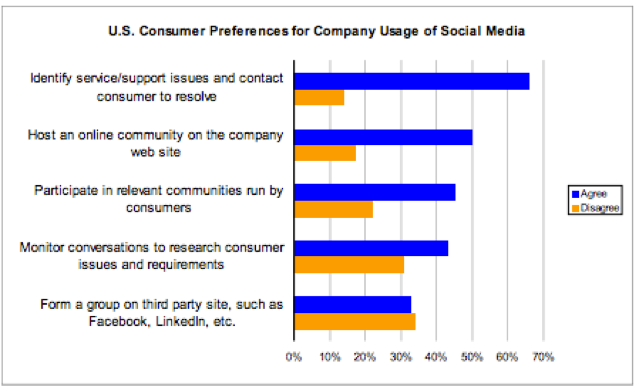
\includegraphics[width=\columnwidth]{images/socialmediause}
\caption{US consumer preferences for company usage of social media~\citep{thompson:2009}}
\label{fig:socialmediause} 
\end{figure}

According to a survey in 2009~\citep{thompson:2009}, more than 60\%,
agrees with the statement that social media have been used as a
technical support for posting technical issues for computer system
(see Figure~\ref{fig:socialmediause}). Our data set was generated from
interactions between users and complex scholarship system for EU
funds. The whole set consists of 391 users and 1390 comment posted by
users as response to system status and reporting their experience with
the system.

Google Analytics have been installed in the web application to track
user’s behavior and web pages’ impressions, however, the data from
Google analytics have been used to identify the server’s status and
divided the status to two stages idle, where system had higher number
of sessions and system marked as failure where system had a lower
session engaged. As shown in Figure 2, is an screen shot of google
analytic in one day and clearly shows the drop at 8 pm where the
system has been identified as failure.

\begin{figure}[!ht]
\centering
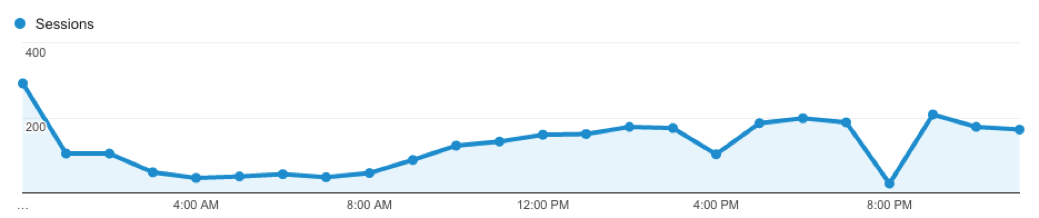
\includegraphics[width=\columnwidth]{images/googleanalytics}
\caption{Google Analytics profile shows behaviour of the system over a
  24 hour period (timeline during the day vs. number of active sessions)}
\label{fig:googleanalytics} 
\end{figure}

\subsection{Personality Insight}

Big Five personality traits (McCrae and John 175-215, 1992) is one of
the most popular models for generally identify how a person is
responsive in the social life. The model, based on the lexical
hypothesis (Crownie 2007), focuses on five dimensions (Digman, J.M,
1990):

\begin{itemize}
\item {\emph{Agreeableness}} is a person's inclination to be humane
  and helpful toward others;
\item {\emph{Conscientiousness}} is a person's being welling to the
  tasks well and in an efficient organised way;
\item {\emph{Extraversion}} is a person's level of socialisation and
  enjoyment of being around people, the higher value means sociable
  person, lower value means person's rather to be alone;
\item {\emph{Neuroticism}} is a person's level to express some
  negative emotions such as anger and stress.
\item {\emph{Openness}} is the measurement of person's level to try
  new things, adventure, imagination.
\end{itemize}

\subsection{Emotion Tones}

The IBM Watson tone analyzer based on Social emotion tones that are being
derived from a research on Emotion Analysis, which is an ensemble
framework to infer emotions from a given text. To derive emotion
scores from text, IBM uses a stacked generalisation-based ensemble
framework to achieve greater predictive accuracy (Costa, Paul T,
1992). Features such as n-grams (unigrams, bigrams and trigrams),
punctuation, emoticons, curse words, greeting words (such as hello,
hi, and thanks), and sentiment polarity are fed into state-of-the
machine learning algorithms to classify emotion categories (Fellbaum,
2005).

Most of these prior works are based on the Linguistic Inquiry and Word
Count (LIWC) psycholinguistics dictionary (Tausczik \& Pennebaker,
2010), and (Pennebaker et al., 2007.) The LIWC is used to find
psychologically meaningful word categories from word usage in writing.


\section{Data Analysis \& Feature Extraction}

\subsection{Overview of the Data}

All interactions have been gathered and grouped by server status and
applied IBM Watson algorithm to fetch the emotion social tone for an
overview of the system behavior and user’s corresponding’s with
Facebook in same time. Figure~\ref{fig:emotiontone} shows the
relationship between the server behavior and emotions of the users, in
the system failed status shows significate difference in overall anger
in different status, furthermore, the Joy parameter shows a
significate difference in system working idle and failure status,
however fear and sadness parameters is almost the same even with the
system idle and working in stable stage.

\begin{figure}[!ht]
\centering
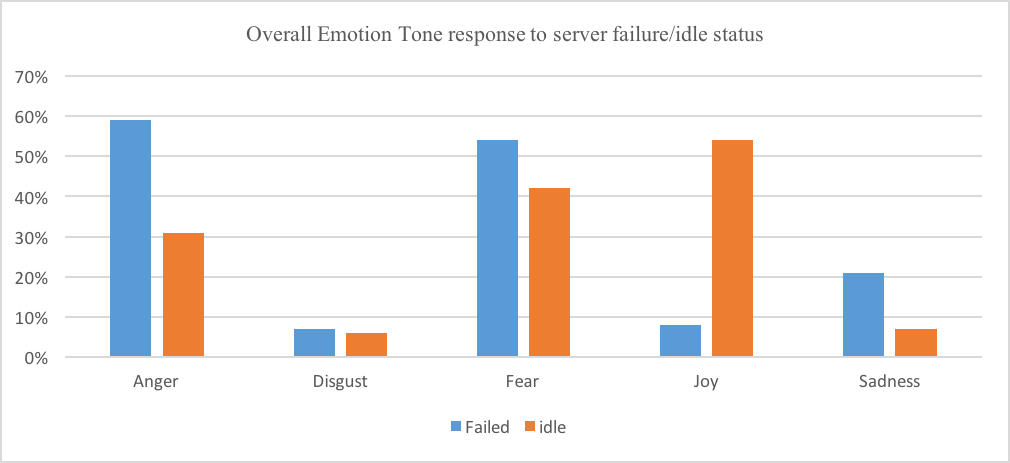
\includegraphics[width=\columnwidth]{images/emotiontone}
\caption{Overall emotion tone response to server failure/idle status}
\label{fig:emotiontone} 
\end{figure}

Identifying user’s personality based on the Facebook interaction
analysis, by applying IBM Watson personality insight tool, by
gathering all comments from user. However, some user’s in the data set
had undertaken the BIG Five (44 questionnaire), in this case these
values have been used instead.

Second stage was grouping the comments based on server status and
segment these interactions by user, to investigate the impact of
server status in the emotion of the user and investigate the BIG Five
dimension as constant parameter.

Investigating the relationship between personality trait dimension and
the social emotion tones, to find the highest correlation to identify
the key elements of the potential model. Applying the linear
regression and Pearson correlation. Building a neural network
multilayer perception using the potential key elements with higher
correlations.

The previous overview encourages more investigation to understand the
relationship between user’s behavior and computer system
behavior’s. The data collected from the social media interactions have
been grouped by users and IBM Watson Personality Insights have been
used to identify BIG Five personality traits for each user. Using IBM
Watson Tone Analyzer, the data been grouped by user’s comments and
server status (failure, idle) to identify user’s social emotion tone
for each user. Table 2, shows sample of data used in the analysis,
while each row represents a separate user, each column represents BIG
5 traits, Social Emotion Tones and Server status. 

\subsection{Statistical Analysis}

The aim of this paper is to model the user’s responsive behavior, one
of the approaches to build a conceptual framework model is to apply
linear regression in Investigating the relationship between BIG 5
personality dimensions and the emotion tones features. 


\begin{figure}[!ht]
\centering
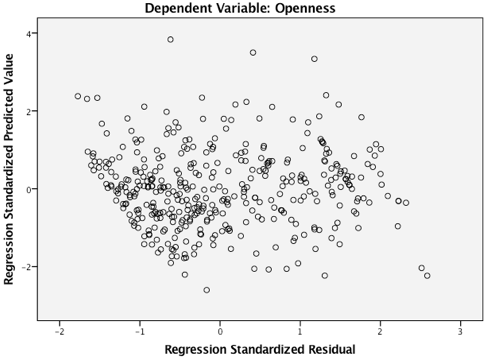
\includegraphics[width=0.45\columnwidth]{images/opennessplot.png}
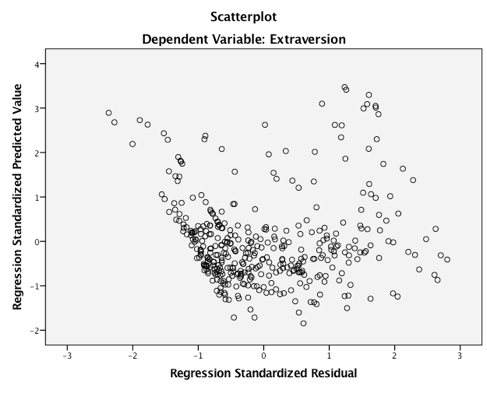
\includegraphics[width=0.45\columnwidth]{images/extraversionplot.png}\\
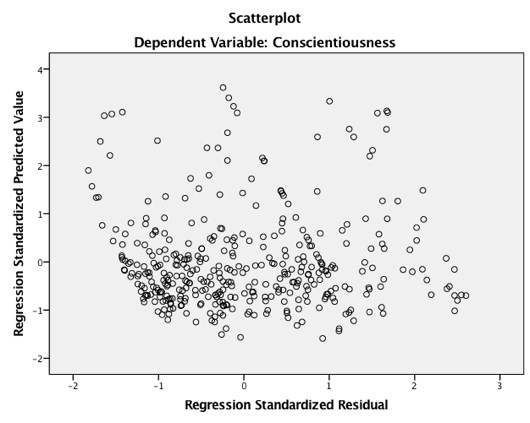
\includegraphics[width=0.45\columnwidth]{images/conscientiousnessplot.png}
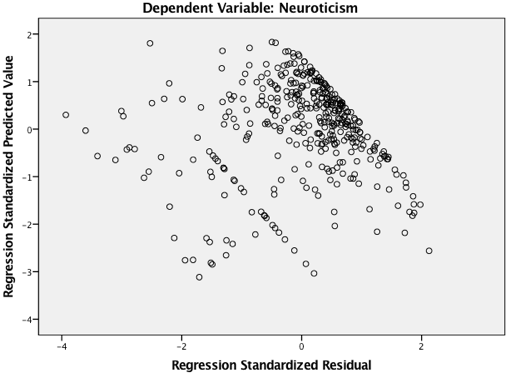
\includegraphics[width=0.45\columnwidth]{images/neuroticismplot.png}\\
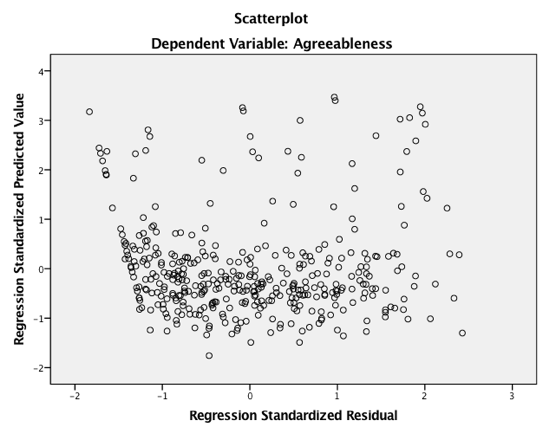
\includegraphics[width=0.45\columnwidth]{images/agreeablenessplot.png}
\caption{Scatterplots of dependent variables of BIG Five dimension and Independent variables are social emotion tones}
\label{fig:scatterplots} 
\end{figure}

% \begin{table}
% \centering
% \begin{tabularx}{\columnwidth}{l Y Y Y Y Y Y Y Y Y Y}
% %\begin{tabular}{c c c} 
% \hline
% & Openness & Extraversion & Consciousness & Agreeableness & Neuroticism\\ 
% \hline
% %\end{tabular}
% \end{tabularx}
% \caption{}

%\end{table}


\begin{table}[!ht]
\centering
\resizebox{\columnwidth}{!}{%

\begin{tabular}{@{}llll|lll|lll|lll|lll@{}}
%\begin{tabularx}{\textwidth}{llll|lll|lll|lll|lll}
\toprule
& \multicolumn{3}{c}{Openness} & \multicolumn{3}{c}{Extraversion} &
\multicolumn{3}{c}{Conscientiousness} &
\multicolumn{3}{c}{Agreeableness} & \multicolumn{3}{c}{Neuroticism} \\

\midrule
           
& \multicolumn{1}{c}{B} & \multicolumn{1}{c}{t} &
\multicolumn{1}{c}{Sig} & \multicolumn{1}{c}{B} &
\multicolumn{1}{c}{t} & \multicolumn{1}{c}{Sig} &
\multicolumn{1}{c}{B} & \multicolumn{1}{c}{t} &
\multicolumn{1}{c}{Sig} & \multicolumn{1}{c}{B} &
\multicolumn{1}{c}{t} & \multicolumn{1}{c}{Sig} &
\multicolumn{1}{c}{B} & \multicolumn{1}{c}{t} &
\multicolumn{1}{c}{Sig} \\


(constant) & 0.356                 & 3.282                 & 0.001                   & 0.162                 & 1.642                 & 0.101                   & 0.16                  & 1.623                 & 0.105                   & 0.297      & 2.831     & 0.005    & 0.828          & 9.934   & 0      \\
anger      & -0.063                & -0.735                & 0.463                   & 0.064                 & 0.831                 & 0.406                   & 0.124                 & 1.592                 & 0.112                   & 0.024      & 0.293     & 0.769    & 0.116          & 1.767    & 0.078     \\
disgust    & 0.478                 & 4.354                 & 0                       & 0.114                 & 1.142                 & 0.253                   & 0.255                 & 2.551                 & 0.011                   & -0.061     & -0.574    & 0.566    & -0.363         & -4.303    & 0    \\
fear       & 0.065                 & 0.534                 & 0.594                   & 0.172                 & 1.549                 & 0.122                   & 0.04                  & 0.356                 & 0.722                   & 0.093      & 0.783     & 0.434    & -0.023         & -0.241    & 0.81    \\
joy        & 0.066                 & 0.561                 & 0.575                   & 0.446                 & 4.179                 & 0                       & 0.436                 & 4.058                 & 0                       & 0.188      & 1.652     & 0.099    & -0.487         & -5.39   & 0      \\
sadness    & -0.226                & -2.118                & 0.035                   & -0.185                & -1.906                & 0.057                   & -0.03                 & -0.313                & 0.754                   & 0.014      & 0.132     & 0.895    & 0.233          & 2.841     & 0.005    \\

\bottomrule

%\end{tabularx} 
\end{tabular}%
}
\caption{Linear regression coefficients}
\label{tbl:linreg}
\end{table}

Linear regression does not show high signification correlation between
(Figure~\ref{fig:scatterplots} and Table~\ref{tbl:linreg}) BIG Five
dimension and Social emotion tones, however, there some correlations
can be highlighted and used as key elements for the model at this
stage. Openness and Disgust, is 0.479 correlation
variable. Extraversion and Joy is 0.446 correlation and P-Value is 0
which shows a reasonable correlation. Conscientiousness and Joy with
0.436 correlation and Disgust with 0.255. Agreeableness, does not have
a high impact in the social emotion parameters the highest correlation
is 0.188 with Joy, which can be neglected as an input to the
model. Neuroticism and Disgust -0.363, Joy -0.487 and p-value is zero
is both cases, and Sadness with 0.233. All correlation values $<$ 0.5
however, it is notice that Agreeableness does not have a linear
relationship with any of the social emotion tones, furthermore, the
social emotion tones that have a potential linear relationship are
Disgust, Joy and Sadness since the three tones have a correlation
between $>$ 0.3 and $<$ 0.5.

Previous linear regression analysis suggested that BIG Five dimensions
(Openness, Extraversion, Conscientiousness and Neuroticism) has the
highest correlation with the Social emotion tones (Joy, Sadness and
Disgust). For further analysis, Pearson Correlation implemented in
same data set to compare the output between Pearson correlation and
Linear Regression correlation. Table 2 shows Pearson
correlation. There is no significate correlation in both, however, in
Pearson correlation, Neuroticism has the highest correlation values
across emotion tones, specially (Anger, Joy and Sadness). Joy as
social emotion tones does have a correlation with all BIG Five
dimensions expect for Agreeableness which agrees with the previous
analysis. However, Disgust as social emotion tone does not have a
strong correlation with any of the BIG Five dimensions which is
different from previous analysis. 

\begin{table}[!ht]
\centering
\begin{tabular}{@{}llllll@{}}
\toprule
                  & Anger  & Disgust & Fear   & Joy    & Sadness \\ 
\midrule
Openness          & -0.098 & 0.231   & 0.043  & 0.035  & -0.151  \\
Conscientiousness & -0.111 & -0.001  & -0.113 & 0.267  & -0.19   \\
Extraversion      & -0.175 & -0.077  & -0.071 & 0.349  & -0.291  \\
Agreeableness     & -0.068 & -0.089  & -0.027 & 0.14   & -0.069  \\
Neuroticism       & 0.375  & -0.037  & 0.153  & -0.488 & 0.379   \\ 

\bottomrule
\end{tabular}
\caption{Pearson correlations}
\label{tab:pearson}
\end{table}


\subsection{Key Elements of the Model}

According to the output of previous two analysis Linear Regression and
Pearson Correlation, the dimension to be identified as the key
elements from the personality traits are (Openness, Extraversion,
Conscientiousness and Neuroticism), the two analysis agrees the
Agreeableness does not have a significate correlation across any
social emotion tone. However, for the social emotion tones to be used
key input elements for the proposed model are (Joy, Sadness, Anger and
Disgust) although Anger tone did not show any significate correlation
in linear regression analysis, however, value of the Pearson
correlation coefficient between 0.3 and 0.5 which can be used as input
for the model.

% insert table 3

The data set used to build this model is consisting of 391 users and 8
inputs (Openness, Extraversion, Conscientiousness, Neuroticism, Joy,
Sadness, Anger and Disgust), the class/output variable is the server
status while (No: System Failed) and (Yes: System idle). The total
number of the instances for testing set is 57. The output of the model
shows a 75.44\% corrected predicted instances and 24.56\% incorrectly
classified instances. The output date encourages more analysis and
research in same direction with expanding the data set.



\section{Conclusions and Future Work}\label{conclusions}

This paper represents an ongoing research (Oatley, T. Crick and
M. Mostafa, 2015) in an attempt to profile user’s digital behavior,
where authors believes that this will help to improve users experience
and computer system architecture. Nowadays, social media is not only
used as sharing platform, it is also used as technical support
platform for various of different computer applications and service
provided. This paper demonstrates the analysis of one of the
web-application platform that have been used Facebook as technical
support platform for their users, and during the usage of the system a
Google analytics used to identify the status of the system in order to
group interactions into two different set one where the system was
idle and the other one where system were failed.

Social network, provided a pool of data for researches to analysis,
through availability of text as raw data provided by social networks,
text and linguistics analysis encourages researches to participate in
the analysis to understand more about available rich data. Personality
traits dimension and Social emotion tones, is based on ongoing
research in the area of linguistics text and social analysis, and
recently a stable accurate tools have been developed by IBM Watson
team as part of IBM research into the social analysis to provide
researchers with SDK to help integrate linguistic analysis into their
research.

The aim of this paper is to produce a model that can predicate server
status based on personality traits and social emotion tones, by
investigating the linear regression and Pearson correlation to
identifying the key elements to be used as input for the neural
network to build this model (Openness, Extraversion,
Conscientiousness, Neuroticism, Joy, Sadness, Anger and Disgust). The
produced model shows a good potential start for further data analysis,
with 75\% accuracy in predication based on 57 test case.

The outcome of the model produced encourage to investigate further
analysis in same direction with some recommendation in future plans:

\begin{itemize}
\item Expanding the data by gathering more data from same type of interactions (Technical Quires).
\item Divide the data by gender, and investigate the relationship
  between gender and emotion raised by the user in different computer
  system status.
\item Explore different computer events not only limited to (Idle,
  failed), but also include more computer events (account hacker,
  system slow, unexpected error and unsaved data).
\end{itemize}


% \begin{acknowledgement}
% If you want to include acknowledgments of assistance and the like at the end of an individual chapter please use the \verb|acknowledgement| environment -- it will automatically render Springer's preferred layout.
% \end{acknowledgement}

% bib
\bibliographystyle{spmpsci}
\bibliography{ai2016}

\end{document}
